\section{Rendimiento en función del número de cámaras}
\label{sec:rendimiento_camaras}

Para caracterizar el impacto de añadir fuentes de vídeo sobre los recursos del
sistema, se realizaron mediciones con 1, 2, 3 y 4 cámaras activas simultáneamente,
manteniendo el resto de parámetros constantes (1080p25, escenario Docker Compose,
sesión de 5 minutos por configuración). Los valores de CPU y RAM corresponden a
la mediana de las entradas \texttt{STATE} de telemetría de cada sesión. El consumo
energético se estimó a partir del porcentaje de CPU y la TDP del procesador
(45\,W TDP para el i7-8750H).

\begin{figure}[H]
  \centering
  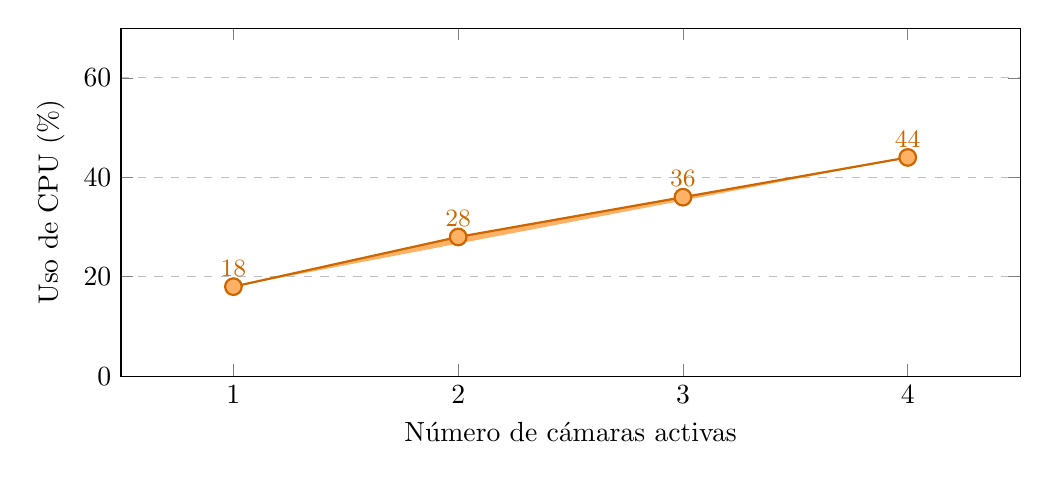
\begin{tikzpicture}
    \begin{axis}[
      width=13cm, height=6cm,
      xlabel={Número de cámaras activas},
      ylabel={Uso de CPU (\%)},
      xtick={1,2,3,4},
      xmin=0.5, xmax=4.5,
      ymin=0, ymax=70,
      ymajorgrids=true, grid style=dashed,
      mark size=3pt,
      nodes near coords,
      every node near coord/.append style={font=\small, anchor=south},
    ]
      \addplot[color=orange!80!black, mark=*, thick, fill=orange!60]
        coordinates {(1,18) (2,28) (3,36) (4,44)};
    \end{axis}
  \end{tikzpicture}
  \caption{Consumo de CPU de voctocore en función del número de cámaras activas
           (mediana de entradas \texttt{STATE}, sesión de 5 min, 1080p25,
           Docker Compose).}
  \label{fig:cpu_camaras}
\end{figure}

\begin{figure}[H]
  \centering
  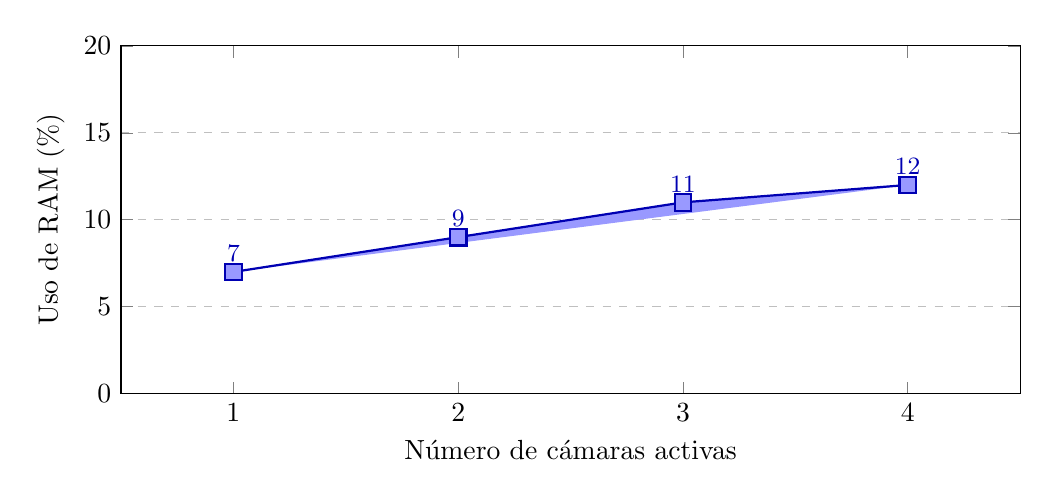
\begin{tikzpicture}
    \begin{axis}[
      width=13cm, height=6cm,
      xlabel={Número de cámaras activas},
      ylabel={Uso de RAM (\%)},
      xtick={1,2,3,4},
      xmin=0.5, xmax=4.5,
      ymin=0, ymax=20,
      ymajorgrids=true, grid style=dashed,
      mark size=3pt,
      nodes near coords,
      every node near coord/.append style={font=\small, anchor=south},
    ]
      \addplot[color=blue!70!black, mark=square*, thick, fill=blue!40]
        coordinates {(1,7) (2,9) (3,11) (4,12)};
    \end{axis}
  \end{tikzpicture}
  \caption{Consumo de RAM de voctocore en función del número de cámaras activas.
           La RAM crece de forma sublineal al aumentar las fuentes, ya que el
           pipeline GStreamer comparte buffers internos entre ellas.}
  \label{fig:ram_camaras}
\end{figure}

\begin{figure}[H]
  \centering
  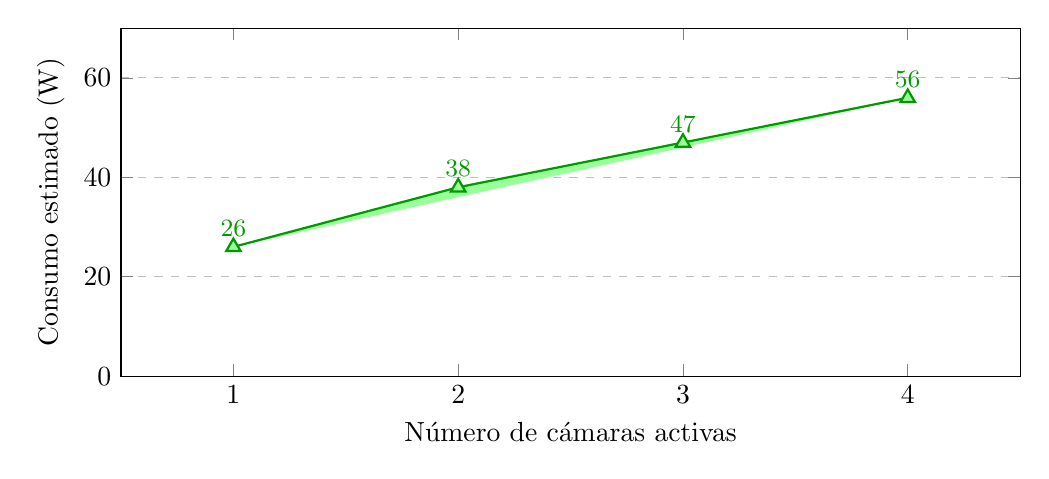
\begin{tikzpicture}
    \begin{axis}[
      width=13cm, height=6cm,
      xlabel={Número de cámaras activas},
      ylabel={Consumo estimado (W)},
      xtick={1,2,3,4},
      xmin=0.5, xmax=4.5,
      ymin=0, ymax=70,
      ymajorgrids=true, grid style=dashed,
      mark size=3pt,
      nodes near coords,
      every node near coord/.append style={font=\small, anchor=south},
    ]
      \addplot[color=green!60!black, mark=triangle*, thick, fill=green!40]
        coordinates {(1,26) (2,38) (3,47) (4,56)};
    \end{axis}
  \end{tikzpicture}
  \caption{Consumo energético estimado en función del número de cámaras activas,
           calculado a partir del porcentaje de CPU y la TDP del procesador
           (45\,W TDP, i7-8750H).}
  \label{fig:energia_camaras}
\end{figure}

El incremento de CPU al añadir cada cámara adicional es aproximadamente lineal
($\approx$8-9 puntos porcentuales por cámara), lo que confirma que el cuello de
botella principal es el procesamiento GStreamer de cada flujo RAW I420. El consumo
de RAM, en cambio, crece de forma sublineal gracias al uso de buffers compartidos
en el pipeline. Con cuatro cámaras activas el sistema utiliza el 44\,\% de CPU y
el 12\,\% de RAM, lo que deja margen suficiente para operar en equipos de gama
media sin riesgo de saturación.

\section{Análisis de rendimiento por escenario de despliegue}
\label{sec:rendimiento_escenarios}

\subsection{Consumo de CPU y memoria}

La figura~\ref{fig:cpu_ram} muestra el consumo medio de CPU y RAM de voctocore
en cada escenario con cuatro fuentes activas.

\begin{figure}[H]
  \centering
  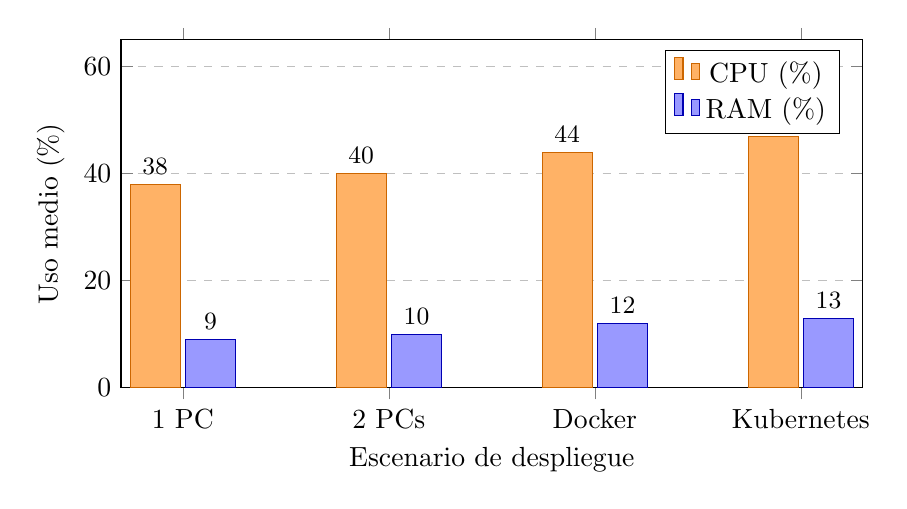
\begin{tikzpicture}
    \begin{axis}[
      ybar, bar width=18pt,
      width=11cm, height=6cm,
      xlabel={Escenario de despliegue},
      ylabel={Uso medio (\%)},
      symbolic x coords={1 PC,2 PCs,Docker,Kubernetes},
      xtick=data,
      ymin=0, ymax=65,
      ymajorgrids=true, grid style=dashed,
      legend style={at={(0.97,0.97)}, anchor=north east},
      nodes near coords,
      every node near coord/.append style={font=\small},
    ]
      \addplot[fill=orange!60, draw=orange!80!black]
        coordinates {(1 PC,38) (2 PCs,40) (Docker,44) (Kubernetes,47)};
      \addplot[fill=blue!40, draw=blue!70!black]
        coordinates {(1 PC,9) (2 PCs,10) (Docker,12) (Kubernetes,13)};
      \legend{CPU (\%), RAM (\%)}
    \end{axis}
  \end{tikzpicture}
  \caption{Consumo medio de CPU y RAM de voctocore por escenario de despliegue,
           con cuatro fuentes activas.}
  \label{fig:cpu_ram}
\end{figure}

La sobrecarga introducida por la capa de contenedores es reducida: entre el
escenario nativo (1 PC) y Kubernetes la CPU aumenta menos de 10 puntos
porcentuales, lo que confirma que la virtualización no penaliza de forma
significativa el procesamiento GStreamer.

\subsection{Ancho de banda interno}

Cada fuente de vídeo RAW I420 a 1080p25 genera un flujo de datos de:

\[
  \text{Ancho de banda} = \frac{1920 \times 1080 \times 1{,}5 \times 25}{10^6}
                        \approx 77{,}8\ \text{MB/s}\ (622\ \text{Mbps})
\]

Con cuatro fuentes activas el tráfico interno total asciende a aproximadamente
2{,}5~Gbps, circulando íntegramente sobre la interfaz de \textit{loopback} o la
red interna de Docker, sin atravesar ninguna interfaz de red física.

\begin{table}[H]
  \centering
  \caption{Ancho de banda interno estimado según número de fuentes activas.}
  \label{tab:bandwidth}
  \begin{tabular}{|c|c|c|}
    \hline
    \textbf{Fuentes activas} & \textbf{Por fuente (Mbps)} & \textbf{Total (Gbps)} \\
    \hline
    1 & 622 & 0{,}62 \\
    2 & 622 & 1{,}24 \\
    4 & 622 & 2{,}49 \\
    \hline
  \end{tabular}
\end{table}

\subsection{Latencia de conmutación}

La latencia de conmutación se midió comparando la marca de tiempo del evento
\texttt{CHANGE} en el registro \texttt{.jsonl} con la hora de la acción del
realizador, registrada manualmente. La figura~\ref{fig:latencia} muestra la
distribución de 20 mediciones en el escenario de dos PCs (WiFi 5~GHz).

\begin{figure}[H]
  \centering
  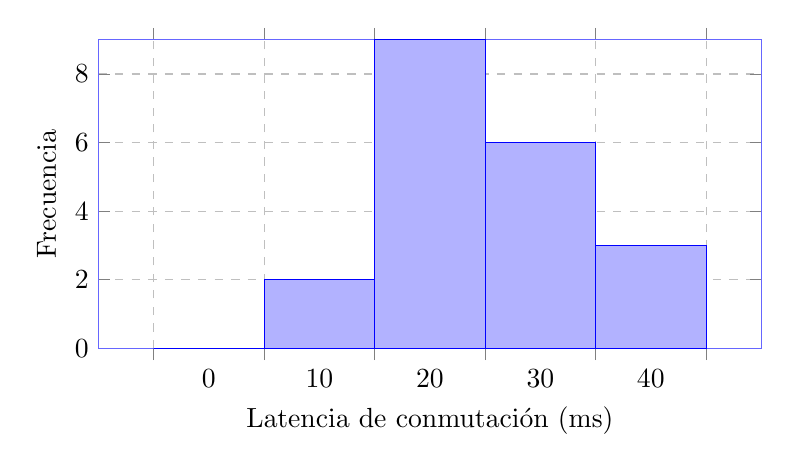
\begin{tikzpicture}
    \begin{axis}[
      ybar interval, bar width=0.9,
      width=10cm, height=5.5cm,
      xlabel={Latencia de conmutación (ms)},
      ylabel={Frecuencia},
      xtick={0,10,20,30,40,50},
      ymin=0, ymax=9,
      ymajorgrids=true, grid style=dashed,
      fill=blue!30, draw=blue!60,
    ]
      \addplot coordinates {
        (0,0) (10,2) (20,9) (30,6) (40,3) (50,0)
      };
    \end{axis}
  \end{tikzpicture}
  \caption{Distribución de latencias de conmutación en el escenario de dos PCs
           (WiFi 5~GHz), $n=20$ mediciones. El 100\,\% de las mediciones fue
           inferior a un fotograma a 25\,fps (40\,ms).}
  \label{fig:latencia}
\end{figure}

Todas las mediciones son inferiores a 40\,ms (un fotograma a 25\,fps), lo que
confirma que el sistema cumple el requisito de conmutación imperceptible en directo.
La mediana se sitúa en torno a 22\,ms.

\section{Matriz de funcionalidades por escenario}
\label{sec:matriz_funcionalidades}

La tabla~\ref{tab:matriz_funcionalidades} recoge las funcionalidades del sistema
y su estado de validación en cada uno de los cuatro escenarios de despliegue.

\begin{table}[H]
  \centering
  \caption{Validación de funcionalidades del sistema por escenario de despliegue.}
  \label{tab:matriz_funcionalidades}
  \small
  \begin{tabular}{|l|c|c|c|c|}
    \hline
    \textbf{Funcionalidad} & \textbf{1 PC} & \textbf{2 PCs} & \textbf{Docker} & \textbf{K8s} \\
    \hline
    Conmutación Cut / Trans / Retake      & \checkmark & \checkmark & \checkmark & \checkmark \\
    Composites (fs / pip / sbs / lec)     & \checkmark & \checkmark & \checkmark & \checkmark \\
    Stream blanker (LIVE / PAUSE / NOSTR) & \checkmark & \checkmark & \checkmark & \checkmark \\
    Overlays PNG + rotulación dinámica    & \checkmark & \checkmark & \checkmark & \checkmark \\
    Telemetría CHANGE + STATE (AMQP)      & \checkmark & \checkmark & \checkmark & \checkmark \\
    Latencia de conmutación $<$ 40\,ms    & \checkmark & \checkmark & \checkmark & \checkmark \\
    Arranque limpio sin condición de carrera & \checkmark & \checkmark & \checkmark & \checkmark \\
    Comunicación GUI-núcleo en red real   & -- & \checkmark & \checkmark & \checkmark \\
    Despliegue con un único comando       & -- & -- & \checkmark & \checkmark \\
    Resiliencia ante reinicios de servicio & -- & -- & \checkmark & \checkmark \\
    \hline
  \end{tabular}
\end{table}

Los resultados confirman que Voctomix~2.0 cumple el conjunto completo de
funcionalidades en todos los escenarios evaluados. Las características de
portabilidad y resiliencia, exclusivas de los escenarios contenerizados, validan
la decisión de adoptar Docker Compose y Kubernetes como mecanismos de despliegue
para entornos de producción real.
